\documentclass[compress]{beamer}

\usetheme{Boadilla}
\usefonttheme[stillsansseriftext]{structurebold}
\usecolortheme{dolphin}
\useoutertheme[subsection=false]{miniframes}
\usepackage{etoolbox}
\usepackage{wrapfig}
\usepackage[english]{babel}
\makeatletter
\patchcmd{\slideentry}{\advance\beamer@xpos by1\relax}{}{}{}
\def\beamer@subsectionentry#1#2#3#4#5{\advance\beamer@xpos by1\relax}%
\makeatother

\begin{document}
\title[Hypothesis Testing] % (optional, only for long titles)
{Doctoral Dissertation Proposal Defense\\Data-adaptive SNP-set-based Association Tests of Longitudinal Traits }
%\subtitle{PH 1915, Fall 2013}
\author[ Yang Yang, M.S] % (optional, for multiple authors)
{Yang Yang, M.S}
\institute[UTSPH] % (optional)
{
  \inst{}%
  UTSPH
}
\date[Dec.15 2014] % (optional)
{Dec 15, 2014}
%\subject{Informatik}


\frame{\titlepage}


\begin{frame}
\frametitle{Table of Contents}
\tableofcontents
\end{frame}


\section{Background}
\frame{\frametitle{Background}
\begin{itemize}
\item Introduction to GWAS
\item Gene-based association test
\item Longitudinal data analysis strategy
\item Gene-set/Pathway based association test
\end{itemize}



}

\subsection{Introduction to GWAS}
%1
  \frame{\frametitle{Introduction to GWAS}
  \framesubtitle{What is SNP?}
\begin{wrapfigure}{l}{0.5\textwidth}
\centering
%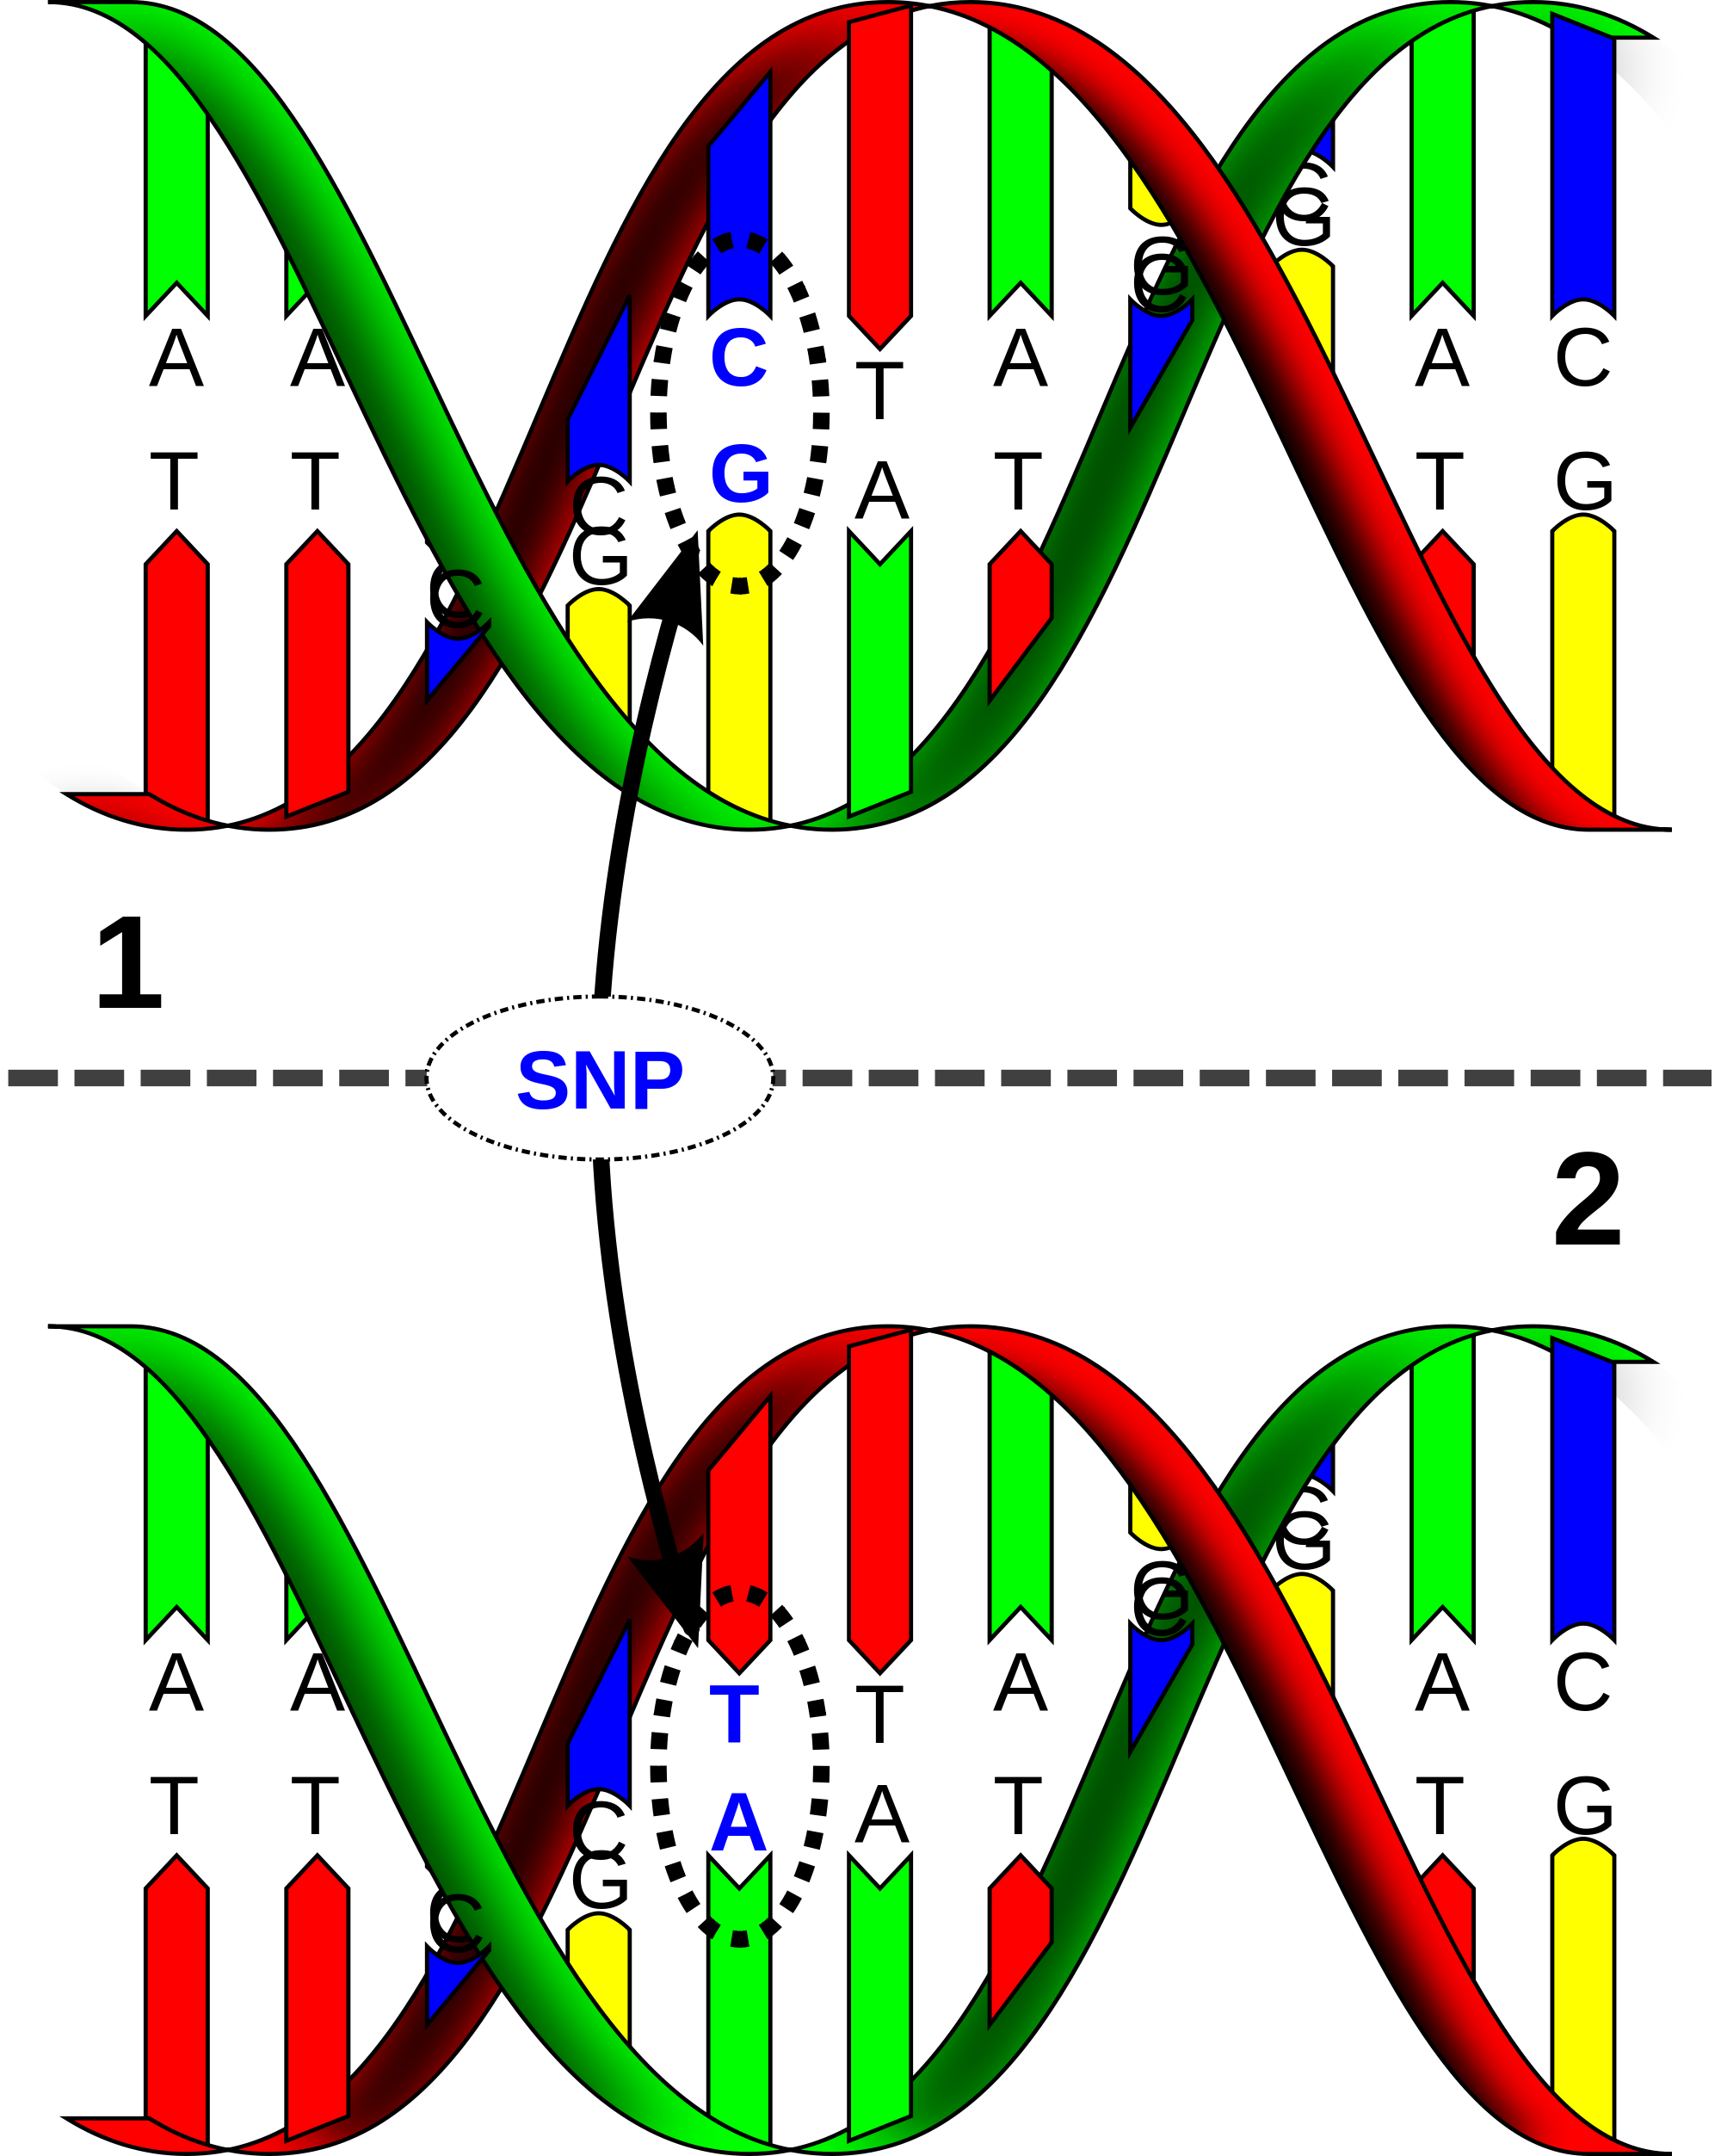
\includegraphics[width=0.8\textwidth]{{{figure/2000px-Dna-SNP.svg}}}
\vspace{-20pt}
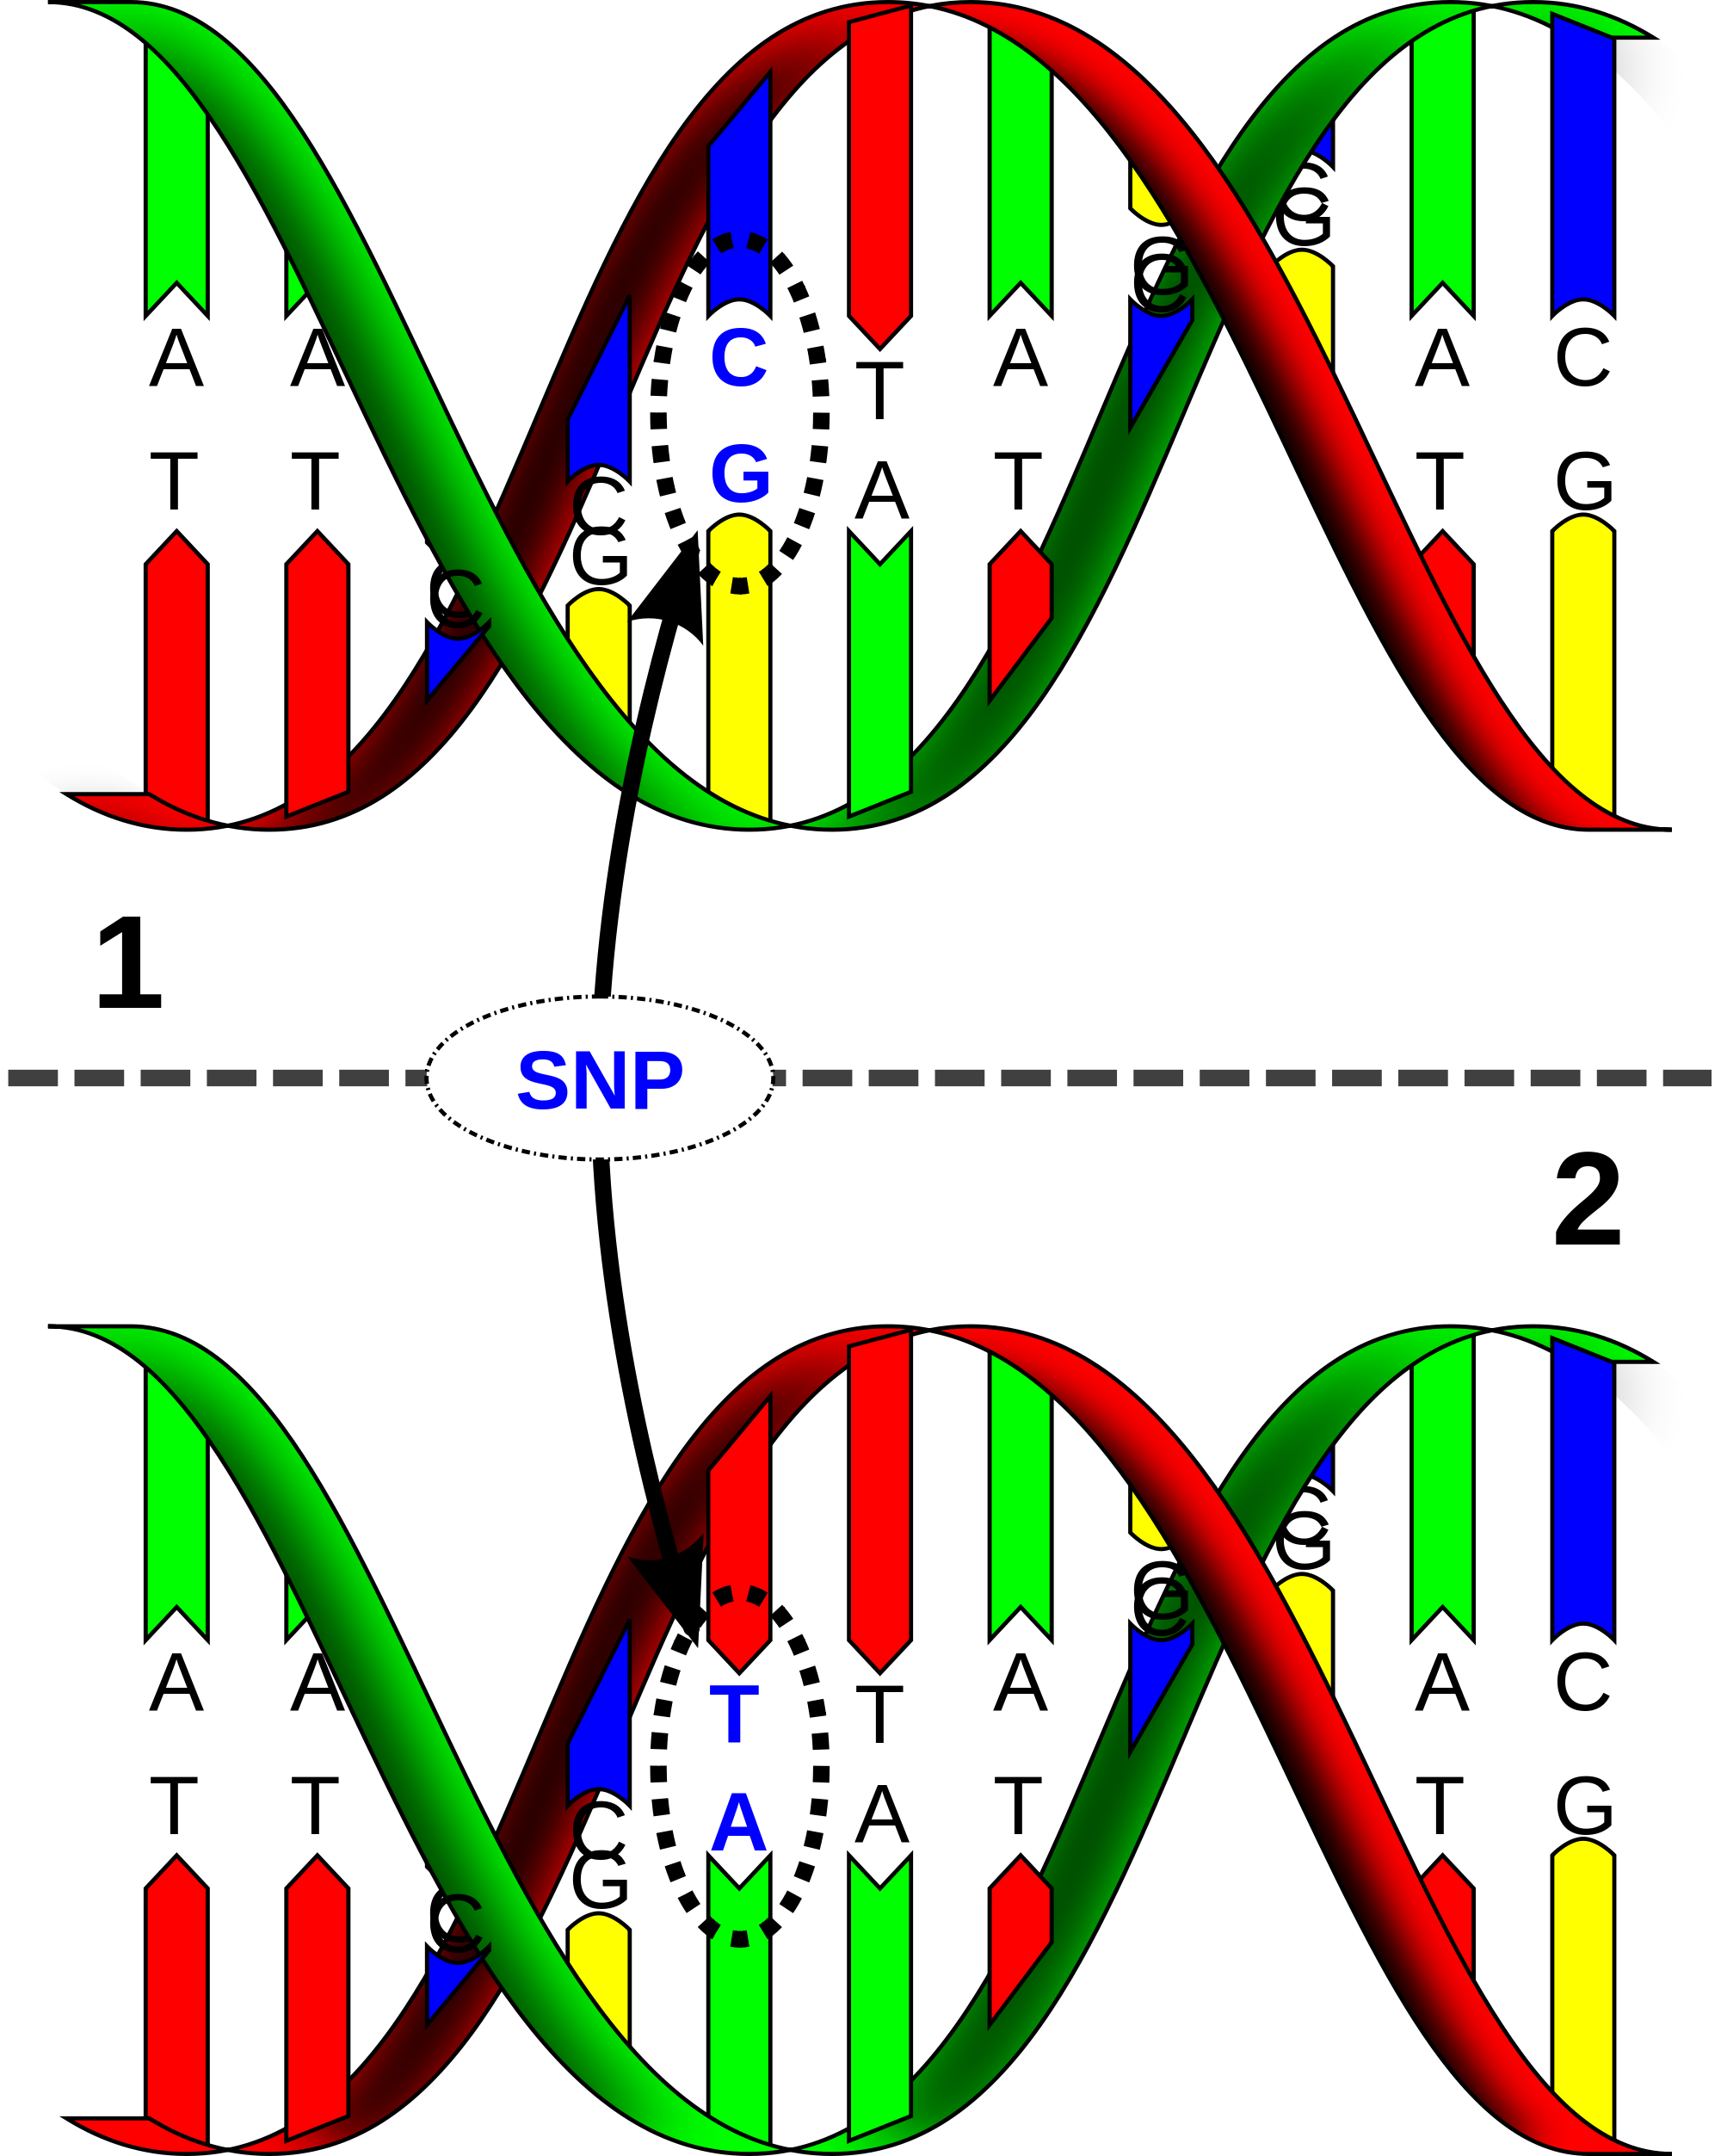
\includegraphics[height=0.6\textheight]{{{figure/2000px-Dna-SNP.svg}}}
%\caption{ single nucleotide polymorphism \label{fig: 2000px-Dna-SNP.svg}}
\end{wrapfigure}
A Single Nucleotide Polymorphism (SNP) is a DNA sequence variation occurring commonly within a population (e.g. 1\%) in which a single nucleotide — A, T, C or G — in the genome (or other shared sequence) differs between members of a biological species or paired chromosomes.
% For example, two sequenced DNA fragments from different individuals, AAGCCTA to AAGCTTA, contain a difference in a single nucleotide. In this case we say that there are two alleles. Almost all common SNPs have only two alleles. The genomic distribution of SNPs is not homogenous; SNPs occur in non-coding regions more frequently than in coding regions or, in general, where natural selection is acting and 'fixing' the allele (eliminating other variants) of the SNP that constitutes the most favorable genetic adaptation.[1] Other factors, like genetic recombination and mutation rate, can also determine SNP density.[2]

}
%%%%%%%%%%%%%%%%%%%%%%%%%%%%%%%%%%%%%%%%
%2
\frame{\frametitle{Introduction to GWAS}
\framesubtitle{A simple flowchart}
\begin{figure}
\vspace{-10pt}
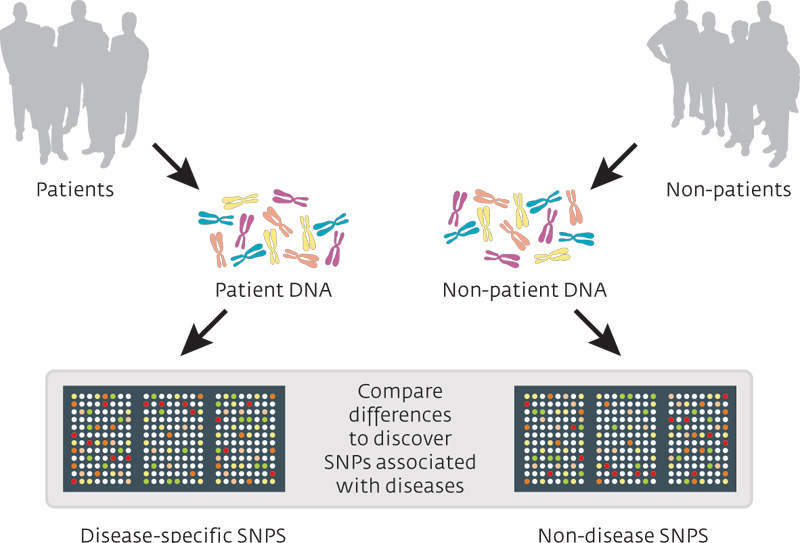
\includegraphics[height=0.6\textheight]{{{figure/gwas_SNPs_casecontrol}}}
%\caption{ single nucleotide polymorphism \label{fig: 2000px-Dna-SNP.svg}}
\end{figure}

}
%%%%%%%%%%%%%%%%%%%%%%%%%%%%%%%%%%%%%%%%
%3
\frame{\frametitle{Introduction to GWAS}
\framesubtitle{A more detailed flowchart}
\begin{figure}
\vspace{-10pt}
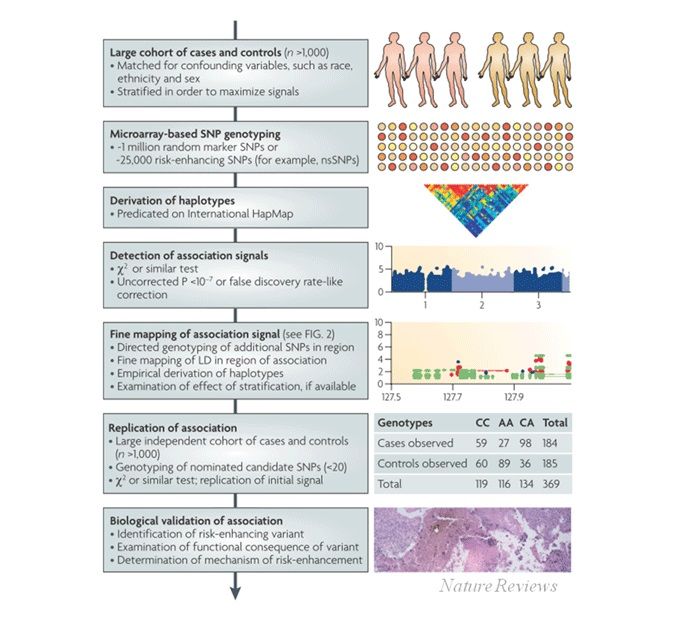
\includegraphics[height=0.8\textheight]{{{figure/gwas_flowchart}}}
%\caption{ single nucleotide polymorphism \label{fig: 2000px-Dna-SNP.svg}}
\end{figure}

}
 
%%%%%%%%%%%%%%%%%%%%%%%%%%%%%%%%%%%%%%%%
%4
\frame{\frametitle{Introduction to GWAS}
\framesubtitle{How does GWAS result look like?}
\begin{figure}
\vspace{-5pt}
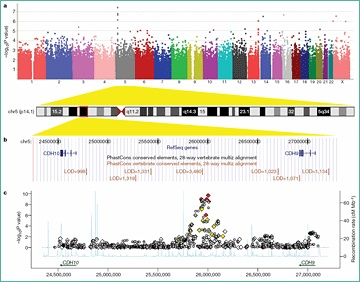
\includegraphics[height=0.8\textheight]{{{figure/GWAS_top10}}}
%\caption{ single nucleotide polymorphism \label{fig: 2000px-Dna-SNP.svg}}
\end{figure}

}

%%%%%%%%%%%%%%%%%%%%%%%%%%%%%%%%%%%%%%%%
%5
\frame{\frametitle{Introduction to GWAS}
\framesubtitle{Common variants and rare variants}
\begin{figure}
\vspace{-5pt}
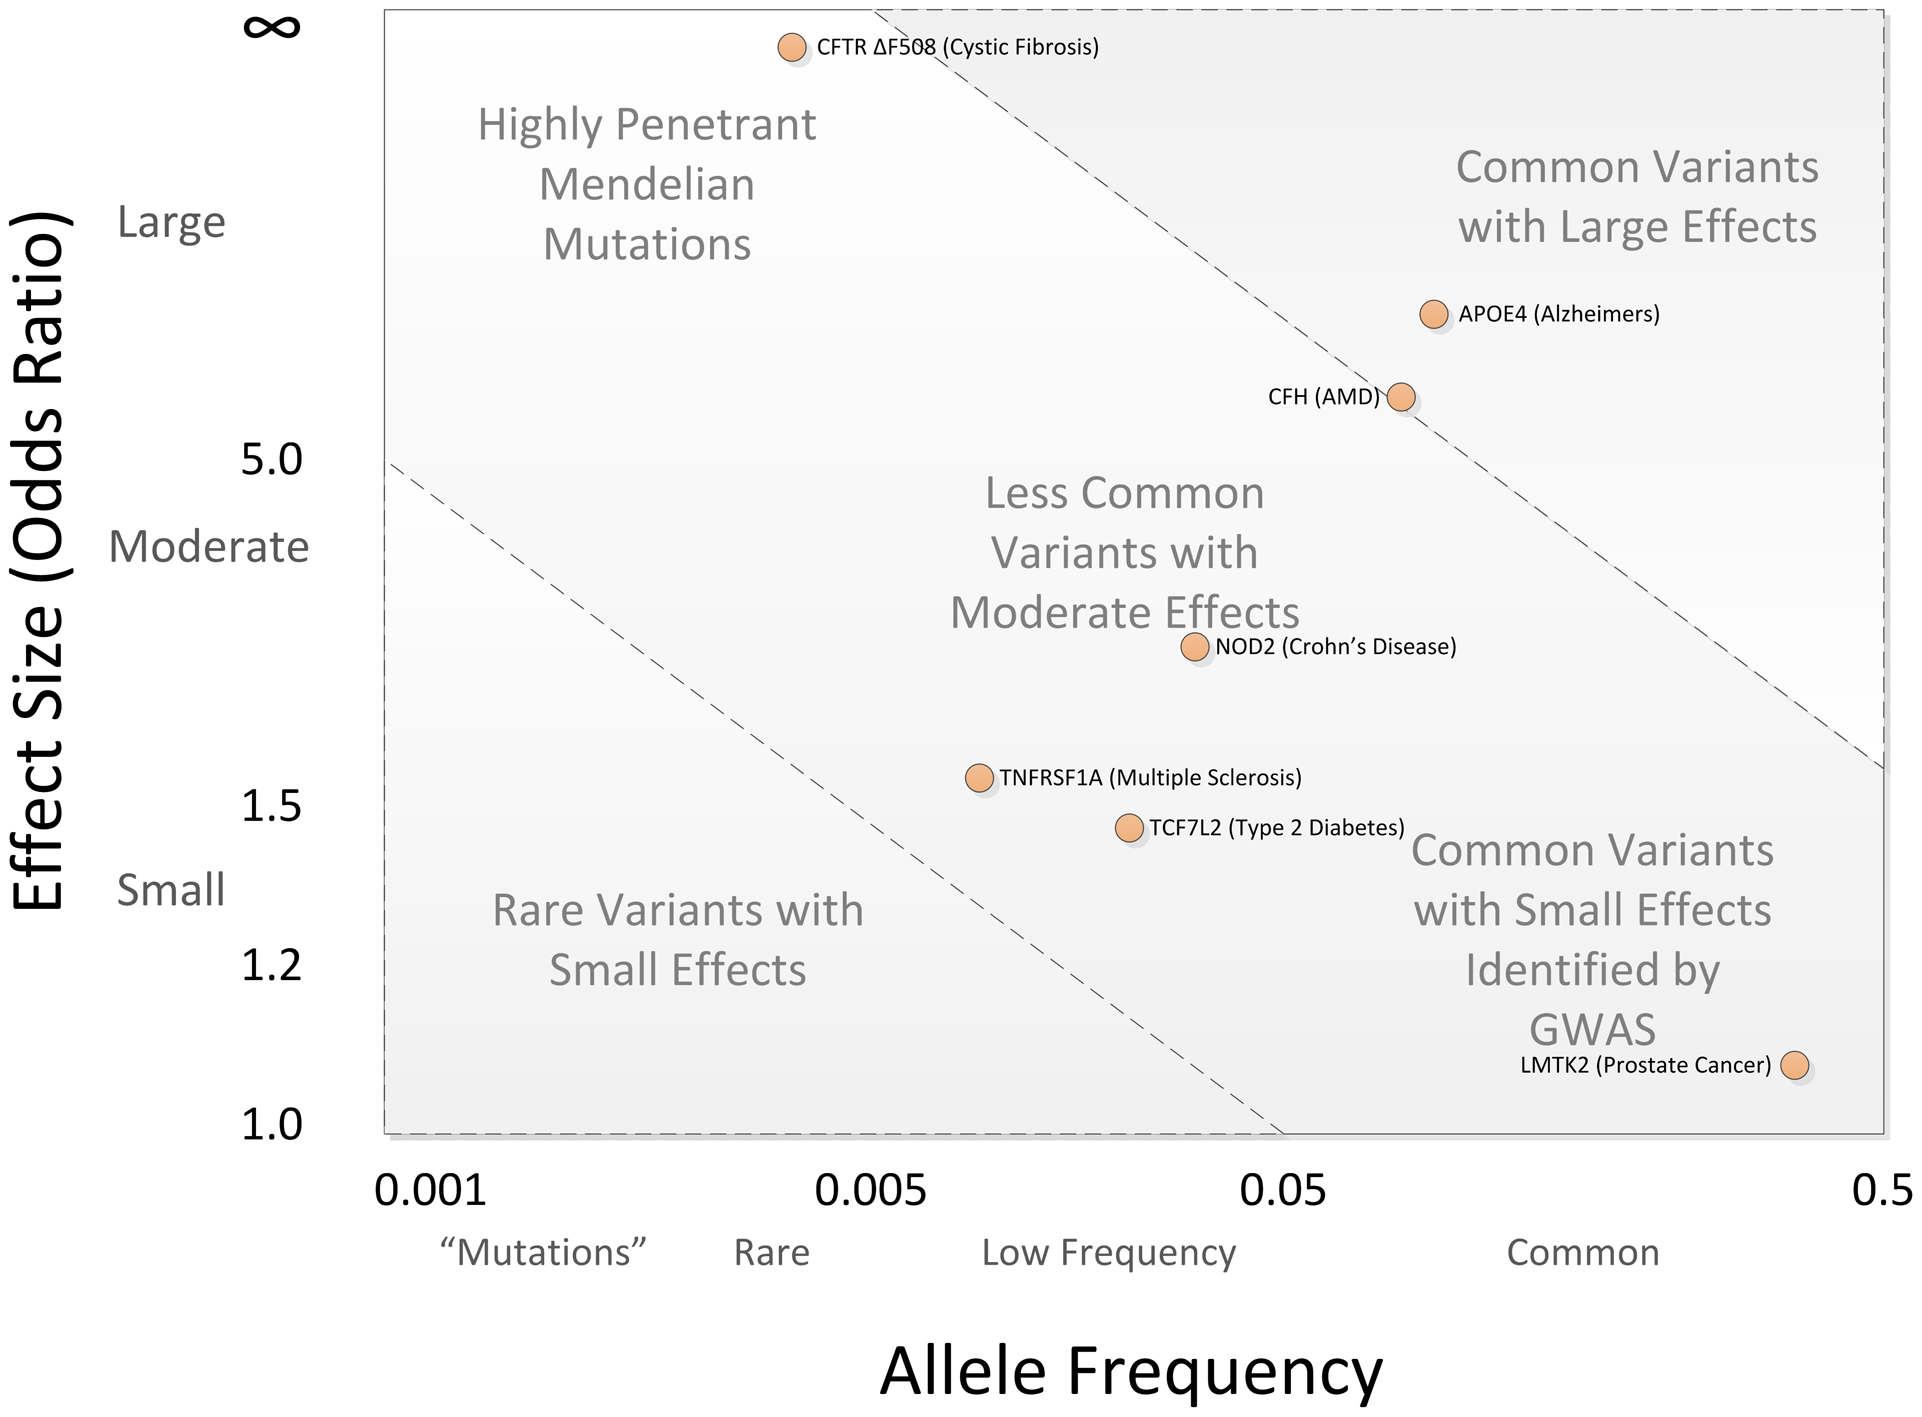
\includegraphics[height=0.8\textheight]{{{figure/GWAS_Disease_allele_effects}}}
%\caption{ single nucleotide polymorphism \label{fig: 2000px-Dna-SNP.svg}}
\end{figure}

}  


\subsection{Gene-based association test}
\frame{\frametitle{Gene-based association test}
\framesubtitle{Common variants and rare variants}
\begin{figure}
\vspace{-5pt}
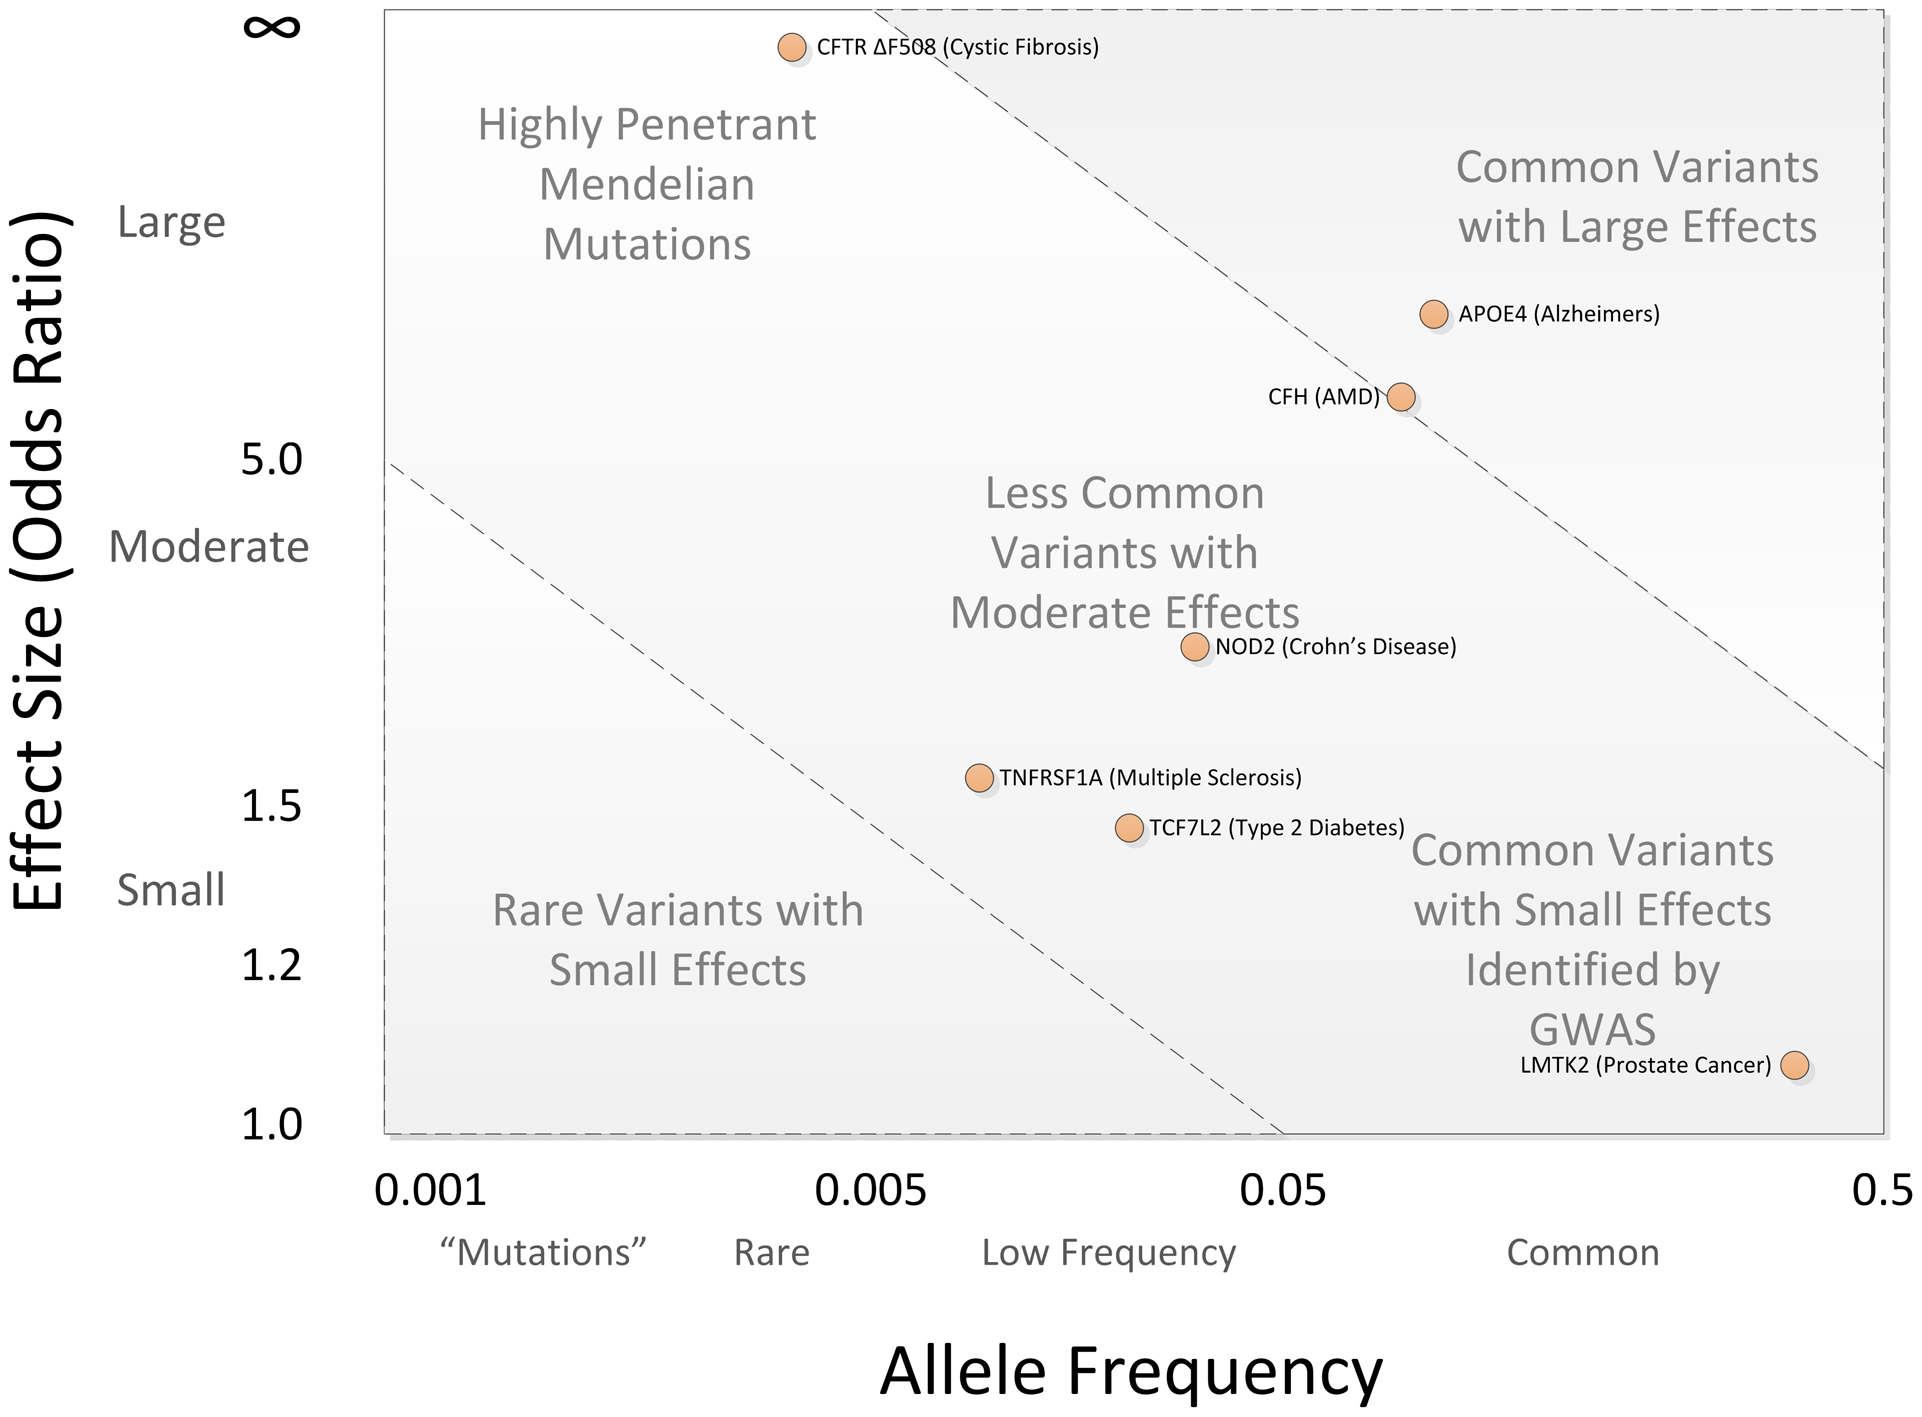
\includegraphics[height=0.8\textheight]{{{figure/GWAS_Disease_allele_effects}}}
%\caption{ single nucleotide polymorphism \label{fig: 2000px-Dna-SNP.svg}}
\end{figure}

}  







%%%%%%%%%%%%%%%%%%%%%%%%%%%%%%%%%%%%%%%%%%
%%%%%%%%%%%%%%%%%%%%%%%%%%%%%%%%%%%%%%%%%%
  
  \frame{\frametitle{Global test}
\small The ANOVA table
 \begin{table}[H]
%\caption{default}
\begin{center}
\begin{tabular}{ccc}
Source of variation & Sum of squares & Degrees of freedom\\
\hline
Regression & SSR($x_1$) & 1\\
& SSR($x_2|x_1$) & 1\\
& \vdots & \vdots\\
& SSR($x_k|x_{k-1},x_{k-2},\cdots,x_1$)&1\\
& SSR & k\\
\hline
Error & SSE & n-(k+1)\\
\hline
Total & SST & n-1
\end{tabular}
\end{center}
\label{default}
\end{table}%
where\\
\small $SSR=SSR(x_1)+SSR(x_2|x_1)+\cdots+SSR(x_k|x_{k-1},x_{k-2},\cdots,x_1)=\hat{\boldsymbol{\beta}}'{\bf X'y}-n\bar{y}^2$\\
$SSE={\bf y'y}-\hat{\boldsymbol{\beta}}'{\bf X'y}$ (for the full model)\\
$SST={\bf y'y}-n\bar{y}^2$ (stays the same for all models)
  }
  
  \frame{\frametitle{Global test}
  Under the null hypothesis, $SSR/\sigma^2\sim \chi_k^2$ and $SSE/\sigma^2\sim \chi_{n-k-1}^2$ are independent. Therefore we have 
  \[TS=\frac{SSR/k}{SSE/(n-k-1)}\sim F_{k,n-k-1}\]
$p-value=Pr(F_{k,n-k-1}>TS)$.
  
  }
  
  \frame{\frametitle{Global test}
Example: \[mgp_i=\beta_0+hp_i\beta_1+wt_i\beta_2+\varepsilon_i\]
$H_0:\beta_1=\beta_2=0$, $H_1$:at least one $\beta\ne0$
  % latex table generated in R 3.0.2 by xtable 1.7-1 package
% Sun Nov  3 11:01:32 2013
\begin{table}[ht]
\centering
\begin{tabular}{lrrrrr}
  \hline
 & Df & Sum Sq & Mean Sq & F value & Pr($>$F) \\ 
  \hline
hp & 1 & 678.37 & 678.37 & 100.86 & 0.0000 \\ 
  wt & 1 & 252.63 & 252.63 & 37.56 & 0.0000 \\ 
  Residuals & 29 & 195.05 & 6.73 &  &  \\ 
   \hline
\end{tabular}
\end{table}
\[TS=\frac{(678.37+252.63)/2}{195.05/29}=69.21>F_{2,29,0.95}=3.33\]
Thus, we reject the null at 0.05 significance level and conclude that at least one $\beta_1$ and $\beta_2$ is not equal to 0.
  } 
  
  
\begin{frame}[fragile]\frametitle{Global test}
Example cont.\\[0.5cm]

The overall F statistic is also available from the output of \verb'summary()' 
\tiny\begin{verbatim}
> summary(fit.all)

Call:
lm(formula = mpg ~ hp + wt, data = mtcars)
Residuals:
   Min     1Q Median     3Q    Max 
-3.941 -1.600 -0.182  1.050  5.854 

Coefficients:
            Estimate Std. Error t value Pr(>|t|)    
(Intercept) 37.22727    1.59879  23.285  < 2e-16 ***
hp          -0.03177    0.00903  -3.519  0.00145 ** 
wt          -3.87783    0.63273  -6.129 1.12e-06 ***
---

Signif. codes:  0 �***� 0.001 �**� 0.01 �*� 0.05 �.� 0.1 � � 1

Residual standard error: 2.593 on 29 degrees of freedom
Multiple R-squared:  0.8268,	Adjusted R-squared:  0.8148 
F-statistic: 69.21 on 2 and 29 DF,  p-value: 9.109e-12
\end{verbatim}
\end{frame}  
  
\subsection{Test of a single covariate} %%%%%%%%%%%%
\frame{\frametitle{Testing of single $\beta_j$}
Once we have determined that at least one of the regressors is important, a natural next question might be which one(s)?\\[0.4cm]

\noindent Important considerations:
\begin{itemize}
\item Is the increase in the regression sums of squares sufficient to warrant an additional predictor in the model?
\item Additional predictors will increase the variance of $\hat{y}$ - include only predictors that explain the response (note: we may not know this through hypothesis testing as confounders may not test significant but would still be necessary in the regression model).
\item Adding an unimportant predictor may increase the residual mean square thereby reducing the usefulness of the model.
\end{itemize}
 }

\frame{\frametitle{Testing of single $\beta_j$}

\[y_i=\beta_0+x_{i1}\beta_1+\cdots+\textcolor{red}{x_{ij}\beta_j}+\cdots+x_{ik}\beta_k+\varepsilon_i\]

\begin{itemize}
\item Question to answer: does one particular variable of interest significantly affect the prediction of {\bf y} when the other independent variables presented in the model?
\item $H_0: \beta_j=0$,
$H_1: \beta_k\ne0$
\item $TS=\frac{\hat{\beta}_j}{\hat{se}(\hat{\beta}_j)}\sim t_{n-k-1}$, reject $H_0$ if $|TS|>t_{n-k-1,1-\alpha/2}$
\item This is a {\bf partial test} because $\hat{\beta}_j$ depends on all of the other predictors $x_i$, for $i\ne j$, that are in the model. Thus, this is a test of the contribution of $x_j$ given other predictors in the model.
\end{itemize}
 }


\begin{frame}[fragile]\frametitle{Testing of single $\beta_j$}
Example cont.: \[mgp_i=\beta_0+hp_i\beta_1+wt_i\beta_2+\varepsilon_i\]
$H_0:\beta_2=0$, $H_1:\beta_2\ne0$\\[0.3cm]
From the summary of lm $\hat{\beta}_2=-3.88$, the variance and covariance matrix of the parameter estimates is 
{\tiny\begin{verbatim}
> vcov(fit.all)
              (Intercept)            hp          wt
(Intercept)  2.5561215917  1.484701e-04 -0.73594515
hp           0.0001484701  8.153566e-05 -0.00376369
wt          -0.7359451464 -3.763690e-03  0.40035167
\end{verbatim}}
\[TS=\frac{-3.88}{\sqrt{0.40}}=-6.13< t_{29,0.025}=-2.05\]
Thus, we reject the null and conclude that $\beta_2\ne0.$
\end{frame}


\subsection{Test of a group of covariates} %%%%%%%%%%
\frame{\frametitle{Testing of a subset of $\boldsymbol{\beta}$}
\[y_i=\beta_0+x_{i1}\beta_1+\cdots+\textcolor{red}{x_{ij}\beta_j+\cdots+x_{ip}\beta_{p}}+\cdots+x_{ik}\beta_k+\varepsilon_i\]
\begin{itemize}
\item Often it is of interest to determine whether a group of predictors contribute to predicting $y$ given another predictor or group of predictors that are in the model. 
\item $H_0:\beta_j=\cdots=\beta_{p}=0$, $H_1: \beta_l\ne0$ for at least one $l, l=j,\cdots,p$
\end{itemize}
} 

\frame{\frametitle{Testing of a subset of $\boldsymbol{\beta}$}
Partition the vector of regression coefficient and {\bf X} matrix as \small\[\boldsymbol{\beta}=\begin{bmatrix}\boldsymbol{\beta}_1\\\boldsymbol{\beta}_2\end{bmatrix}, {\bf X}=[{\bf X_1}|{\bf X_2}]\]

Hypotheses of interest: $H_0: \boldsymbol{\beta}_2=0$ v.s. $H_1: \boldsymbol{\beta}_2\ne0$\\[0.4cm]

The model can be written as ${\bf y}={\bf X_1}\boldsymbol{\beta}_1+{\bf X_2}\boldsymbol{\beta}_2+\boldsymbol{\varepsilon}$
\small\[SSR({\bf X})=\boldsymbol{\hat{\beta}'{\bf X}'{\bf y}}\ (k+1 \mbox{ degrees of freedom})\]
\small\[MSE=\frac{{\bf y'y}-\boldsymbol{\hat{\beta}'{\bf X}'{\bf y}}}{n-k-1}\]
\small\begin{eqnarray*}SSR({\bf X_2}|{\bf X_1})&=&SSR({\bf X})-SSR({\bf X_1})\\
&=&SSE(reduced)-SSE(full)\ (r \mbox{ degrees of freedom})\end{eqnarray*}
Under $H_0$
\[TS=\frac{SSR({\bf X_2}|{\bf X_1})/r}{MSE}\sim F_{r,n-k-1}\]
}

\begin{frame}[fragile]\frametitle{Testing of a subset of $\boldsymbol{\beta}$}
Example cont.
\[mgp_i=\beta_0+disp_i\beta_1+hp_i\beta_2+qsec_i\beta_3+wt_i\beta_4+\varepsilon_i\]
\tiny\begin{verbatim}
fit.sub<-lm(mpg~disp+hp+qsec+wt,data=mtcars)
> summary(fit.sub)

Call:
lm(formula = mpg ~ disp + hp + qsec + wt, data = mtcars)

Residuals:
    Min      1Q  Median      3Q     Max 
-3.8664 -1.5819 -0.3788  1.1712  5.6468 

Coefficients:
             Estimate Std. Error t value Pr(>|t|)   
(Intercept) 27.329638   8.639032   3.164  0.00383 **
disp         0.002666   0.010738   0.248  0.80576   
hp          -0.018666   0.015613  -1.196  0.24227   
qsec         0.544160   0.466493   1.166  0.25362   
wt          -4.609123   1.265851  -3.641  0.00113 **
---
Signif. codes:  0 �***� 0.001 �**� 0.01 �*� 0.05 �.� 0.1 � � 1

Residual standard error: 2.622 on 27 degrees of freedom
Multiple R-squared:  0.8351,	Adjusted R-squared:  0.8107 
F-statistic: 34.19 on 4 and 27 DF,  p-value: 3.311e-10
\end{verbatim}
\end{frame}

\begin{frame}[fragile]\frametitle{Testing of a subset of $\boldsymbol{\beta}$}
$H_0:\beta_1=\beta_2=\beta_3=0$, $H_1:\beta_j\ne0,j=1,2,3$\\[0.3cm]
% latex table generated in R 3.0.2 by xtable 1.7-1 package
% Sun Nov  3 15:30:35 2013
{\scriptsize\begin{table}[ht]
\centering
\begin{tabular}{lrrrrr}
  \hline
 & Df & Sum Sq & Mean Sq & F value & Pr($>$F) \\ 
  \hline
disp & 1 & 808.89 & 808.89 & 117.65 & 0.0000 \\ 
  hp & 1 & 33.67 & 33.67 & 4.90 & 0.0356 \\ 
  qsec & 1 & 6.71 & 6.71 & 0.98 & 0.3321 \\ 
  wt & 1 & 91.15 & 91.15 & 13.26 & 0.0011 \\ 
  Residuals & 27 & 185.64 & 6.88 &  &  \\ 
   \hline\\[0.2cm]

% latex table generated in R 3.0.2 by xtable 1.7-1 package
% Sun Nov  3 16:26:46 2013

  \hline
 & Df & Sum Sq & Mean Sq & F value & Pr($>$F) \\ 
  \hline
wt & 1 & 847.73 & 847.73 & 91.38 & 0.0000 \\ 
  Residuals & 30 & 278.32 & 9.28 &  &  \\ 
   \hline
\end{tabular}
\end{table}
}

{\small\begin{eqnarray*}
SSR(disp,hp,qsec|wt)=278.32-185.64=92.68
\end{eqnarray*}
\[TS=\frac{92.68/3}{6.88}=4.49>F_{3,27,0.95}=2.96\]
Thus we reject the null and conclude that $disp$, $hp$ and $qsec$ are jointly significant.}
\end{frame}



     
\section{Test of the contrast}    
  \frame{\frametitle{Test of the contrast}
  Many functions in R can be used to test the contrasts.
\begin{table}[htdp]
%\caption{default}
\small\begin{center}
\begin{tabular}{p{2.2cm}p{2cm}p{6cm}}
\hline
function&package&description\\
\hline
fit.contrast& \{gmodels\}&Compute and test arbitrary contrasts for regression objects\\
contrast.lm& \{contrast\}&computes one or more contrasts of the estimated regression coefficients\\
glht&\{multcomp\}&generalized linear hypothesis test\\
linear.hypothesis& \{car\}&Generic function for testing a linear hypothesis\\
\hline
\end{tabular}
\end{center}
\label{default}
\end{table}%
A simple example.  
}

  
  
\section{Regression Diagnostics}%%%%%
\frame{\frametitle{Regression Diagnostics}
Frequently used functions provide information used with model diagnostics
\begin{table}[htdp]
%\caption{default}
\begin{center}
\small\begin{tabular}{p{2cm}p{9.5cm}}
fitted.values()&Returns fitted values\\
residuals()&Returns residuals\\
rstandard()&Standardized residuals, variance one; residual standardized using overall error variance (9.25)\\
rstudent()& Studentized residuals, variance one; residual standardized using leave-one-out measure of the error variance (9.26)\\
qqnorm()&Normal quantile plot\\
qqline()&Add a line to the normal quantile plot\\
plot.lm()&Given a lm object it produces six diagnostic plots, selected using the `which' argument; default is plots 1-3 and 5\\
&1.Residual versus fitted values\\
&2. Normal quantile-quantile plot\\
&3. $\sqrt{\mbox{$|$Standardized residuals$|$}}$ versus fitted values\\
&4. Cook's distance versus row labels\\
&5.Standardized residuals versus leverage along with contours of Cook's distance
\end{tabular}
\end{center}
\label{default}
\end{table}% 
}

\frame{
\begin{table}[htdp]
%\caption{default}
\begin{center}
\small\begin{tabular}{p{2.8cm}p{8.8cm}}
plot.lm()&6. Cook's distance versus leverage/(1-leverage) with$\sqrt{|\mbox{Standardized residuals}|}$ contours\\
dffits()&Return DFFITS\\
dfbeta()&Return DFBETAS\\
covratio()&Return covariance ratio; vector whose $i$th element is the ratio of the determinants of the estimated covariance matrix with and without data point $i$\\
cooks.distance()&Returns Cook's distance\\
hatvalues()&Diagonal of the hat matrix\\
influence.measures()&Returns the previous five measure of influence and flags influential points\\
lm.influence()&Returns four measures of influence:\\
\ hat& Diagonal of the hat matrix, measure of leverage\\
\ coefficients& Matrix, whose $i$th row contains the change in the estimated coefficients when the $i$th case is removed\\
\ sigma& Vector, whose $i$th element contains the estimated of the residual standard error when the $i$th case is removed\\
\ wt.res&Vector of weighted residuals or raw residuals if weights are not set.
\end{tabular}
\end{center}
\label{default}
\end{table}% 
} 

\begin{frame}[fragile]\frametitle{Regression Diagnostics}
Example:
\scriptsize\begin{verbatim}
fit<-lm(mpg~wt,data=mtcars)
#influential points are labeled
par(mfrow=c(2,2))
plot(fit)	#returns four diagnostics plot (1-3 and 5)
par(mfrow=c(2,3))
plot(fit,which=1:6)	#returns all six diagnostic plots

par(ask=T)
plot(residuals(fit),fitted.values(fit))
qqnorm(residuals(fit));qqline(residuals(fit))
plot(cooks.distance(fit),rownames(fit),type="h")

#influence measures
influence.measures(fit)

#extract influential points, uses $is.inf
inf.temp<-influence.measures(fit)
inf.pts<-which(apply(inf.temp$is.inf,1,any))
mtcars[inf.pts,]

#Influence measures
lm.influence(fit)
\end{verbatim}
\end{frame}

\begin{frame}[fragile]\frametitle{Regression Diagnostics}
\small\begin{verbatim}
#Extract points that cause the greatest change in the estimates
lm.inf.coef<-lm.influence(fit)$coefficients
lm.inf.pts<-apply(lm.inf.coef[,2,drop=F],2,
+ FUN=function(x)which.max(abs(x)))

lm.inf.coef[lm.inf.pts,] 
#this gives the same results with the diagnostic plots

#Get the five points that cause the greatest 
#change in the estimates
lm.inf.pts.top5<-apply(lm.inf.coef,2, 
+ FUN=function(x)names(rev(sort(abs(x)))[1:5]))
lm.inf.pts.top5
\end{verbatim}
\end{frame}

\section{Appendix}
\subsection{Types of sums of squares}
\frame{\frametitle{Sums of Squares}
\begin{itemize}
\item {\scriptsize Type I}
\begin{itemize}{\scriptsize
\item Also called "sequential" sum of squares
\item Can be viewed as the reduction in SSE obtained by adding additional term to a fit that already includes the terms listed before it.
\item Pros: a complete decomposition of the predicted SS for the whole model; Preferable when some factors should be taken out before other factors.
\item Cons:Lack of invariance to order of entry into the model; not appropriate for factorial designs.
}\end{itemize}

\item {\scriptsize Type II}
\begin{itemize}{\scriptsize
\item The reduction in SSE due to adding the term to the model after all other terms except those that contain it (interaction terms).
\item Pros: Appropriate for model building and natural choice for regression; Most powerful when no interaction; Invariant to the order when the factors are entered to the model.
\item Cons:Not appropriate for factorial designs
}\end{itemize}

\item {\scriptsize Type III}
\begin{itemize}{\scriptsize
\item Effect of each variable is evaluated after all other factors have been accounted for.
\item Pros: Appropriate for unbalanced data;
\item Cons: Testing main effects when interactions presence; not appropriate with missing cells.
}\end{itemize}
\end{itemize}

}

\subsection{Eqvivalance of LRT and F-test}
\frame{\frametitle{LRT and F test}
{\small The F-test of the null hypothesis $H_0: {\bf C}\boldsymbol{\beta}={\bf t}$ is a likelihood ratio test (LRT) because the F-ratio is a monotone transformation of the likelihood ratio $\lambda$.}\\

{\scriptsize{\em Proof:}\\
The log-likelihood is given by
\begin{eqnarray*}
\log L(\boldsymbol{\beta},\sigma^2)&=&-\frac{n}{2}\log(2\pi)-\frac{n}{2}\log({\sigma}^2)-\frac{1}{2{\sigma}^2}({\bf y-X}\boldsymbol{{\beta}})'({\bf y-X}\boldsymbol{{\beta}})\\
&=&-\frac{n}{2}\log(2\pi)-\frac{n}{2}\log({\sigma}^2)-\frac{1}{2{\sigma}^2}SSE({\bf X})\\
\lambda=-2\log\frac{\max_{H_0}L(\boldsymbol{\beta})}{\max_{H_1 U H_0}L(\boldsymbol{\beta})}&=&-2\log\frac{L(\boldsymbol{\hat{\beta}_1})}{L(\boldsymbol{\hat{\beta}_1,\hat{\beta}_2})}\\
&=&\frac{SSE({\bf X_1})-SSE({\bf X_1+X_2})}{\sigma^2},
\end{eqnarray*}
for a fixed value of $\sigma^2$.\\

Since $\sigma^2$ is unknown, we can use $\hat{\sigma}^2_{MLE}=SSE({X_1+X_2})/n$, then\\
$$F=C*\lambda=\frac{[SSE({\bf X_1})-SSE({\bf X_1+X_2})]/r}{SSE({\bf X_1+X_2})/(n-k-1)}\sim F_{r, n-k-1},$$ where $C=\frac{n-k-1}{nr}$.
}
}

\section{References}
\frame{\frametitle{References}
\begin{enumerate}
\item Elizabeth R. Brown, {\em Introduction to Regression Models}
\item Nicholas Christian, {\em Statistical Computing in R}
\item Langsrud, $\phi$. (2003), ANOVA for Unbalanced Data: Use Type II Instead of Type III Sums of Squares, {\em Statistics and Computing}, 13, 163-167.
\end{enumerate}
}
  
\end{document}